% Preamble
\documentclass[a4paper, 12pt]{article}
\usepackage[margin=1in]{geometry} % Set margin
\usepackage{pdfpages} % Insert pdf pages
\usepackage{amssymb,amsmath,amsthm, amsfonts} % Math libraries

% Custom commands
\newcommand{\sub}[1]{\subsection{\underline{#1}}}
\newcommand{\subsub}[1]{\subsubsection{\underline{#1}}}
\newcommand{\R}{\ensuremath{\mathbb{R}}}
\newcommand{\F}{\ensuremath{\mathbb{F}}}
\newcommand{\N}{\ensuremath{\mathbb{N}}}
\newcommand{\Onef}{\ensuremath{1_{\F}}}
\newcommand{\Zerof}{\ensuremath{0_{\F}}}
\newcommand{\eqbcuz}[1]{\text{~$\stackrel{(#1)}{=}$~}}
\newcommand{\eq}[1]{\begin{align*}#1\end{align*}}
\newcommand{\eqn}[1]{\begin{align}#1\end{align}}
\newcommand{\set}[1]{\big{\{} #1 \big{\}}}
\newcommand{\bigset}[1]{\bigg{\{} #1 \bigg{\}}}
\renewcommand{\qed}{\hfill\(\qedsymbol\)}
\newtheorem{lemma}{Lemma}

% Begin Document %
\begin{document}

% Title Page
\begin{titlepage}
    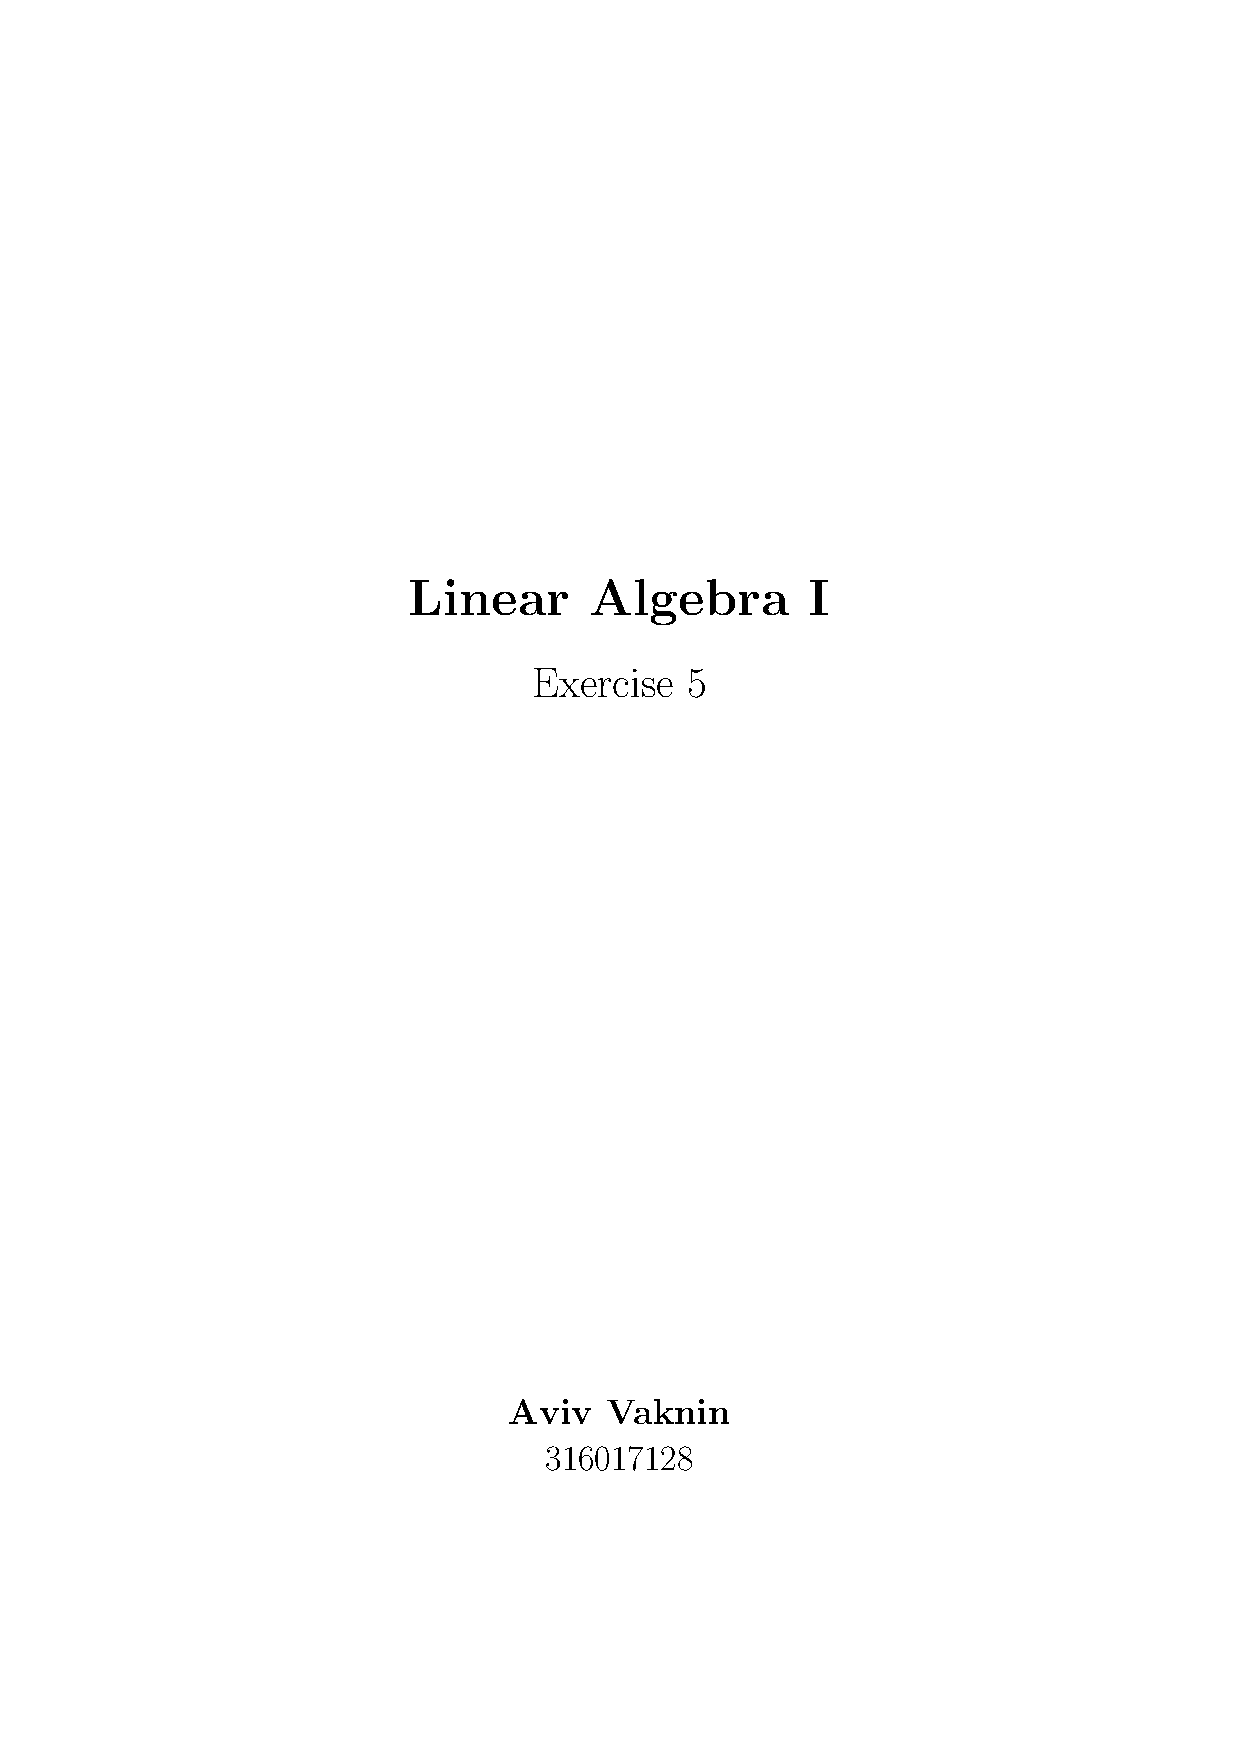
\includepdf{title.pdf}
\end{titlepage}

% 2
\setcounter{section}{1}
\section{}
\sub{Calculate $A^2, B^2, AB$ and $BA$}
\eq{
    A^2=\begin{bmatrix}
        1&2&1&0&0\\
        0&1&2&0&0\\
        0&0&1&0&0\\
        0&0&0&1&2\\
        0&0&0&0&1
    \end{bmatrix}
}
\eq{
    B^2=\begin{bmatrix}
        1&0&2&0&0\\
        0&1&0&0&0\\
        0&0&1&0&0\\
        0&0&0&-1&0\\
        0&0&0&0&-1
    \end{bmatrix}
}
\eq{
    AB=\begin{bmatrix}
        1&1&1&0&0\\
        0&1&1&0&0\\
        0&0&1&0&0\\
        0&0&0&1&-1\\
        0&0&0&1&0
    \end{bmatrix}
}
\eq{
    BA=\begin{bmatrix}
        1&1&1&0&0\\
        0&1&1&0&0\\
        0&0&1&0&0\\
        0&0&0&0&-1\\
        0&0&0&1&1
    \end{bmatrix}
}
\sub{}
\eq{
    A^k=\begin{bmatrix}
        1&k&(A^{k-1}+(k-1))&0&0\\
        0&1&k&0&0\\
        0&0&1&0&0\\
        0&0&0&1&k\\
        0&0&0&0&1
    \end{bmatrix}
}
\eq{
    B^k=\begin{bmatrix}
        1&0&k&0&0\\
        0&1&0&0&0\\
        0&0&1&0&0\\
        0&0&0&x&y\\
        0&0&0&z&w
    \end{bmatrix}
}
When $x,y,z$ and $w$ alternate between $-1, 0$ and $1$.
\pagebreak

% 4.3
\setcounter{section}{4}
\setcounter{subsection}{2}
\sub{Find P, R and show P as a multiplication of elementary matrices}
\eq{
    R=\begin{bmatrix}
        1&0&15\\
        0&1&6\\
        0&0&0\\
        0&0&0
    \end{bmatrix}
}
\eq{
    P=\begin{bmatrix}
        3&0&0&2\\
        1&0&0&1\\
        -1&0&1&1\\
        3&1&0&0
    \end{bmatrix}
}
\eq{
    P=
    \begin{bmatrix}
        1&0&0&0\\
        0&1&0&0\\
        0&1&1&0\\
        0&0&0&1
    \end{bmatrix}
    \begin{bmatrix}
        1&2&0&0\\
        0&1&0&0\\
        0&0&1&0\\
        0&0&0&1
    \end{bmatrix}
    \begin{bmatrix}
        1&0&0&0\\
        0&1&0&0\\
        -2&0&1&0\\
        0&0&0&1
    \end{bmatrix}
    \begin{bmatrix}
        1&0&0&0\\
        1&1&0&0\\
        0&0&1&0\\
        0&0&0&1
    \end{bmatrix}
    \begin{bmatrix}
        1&0&0&0\\
        0&0&0&1\\
        0&0&1&0\\
        0&1&0&0
    \end{bmatrix}
    \begin{bmatrix}
        1&0&0&0\\
        3&1&0&0\\
        0&0&1&0\\
        0&0&0&1
    \end{bmatrix}
}

% 5
\section{Decide whether the matrix is invertible or not.\\If it is invertible, find its inverse.}
\sub{}
$U_1$ is invertible.
\eq{
    U_1^{-1}=\begin{bmatrix}
        \frac{9}{14}&-\frac{1}{14}&-\frac{3}{14}\\
        \frac{10}{7}&-\frac{5}{7}&-\frac{1}{7}\\
        -\frac{6}{7}&\frac{3}{7}&\frac{2}{7}
    \end{bmatrix}
}
\sub{}
$U_2$ is not invertible, because its rref is:
\eq{
    rref(U_2)=\begin{bmatrix}
        1&0&0\\
        0&1&1\\
        0&0&0
    \end{bmatrix}
    \neq{I_3}
}
\sub{}
$U_3$ is not invertible, because its rref is:
\eq{
    rref(U_3)=\begin{bmatrix}
        1&0&1\\
        0&1&0\\
        0&0&0
    \end{bmatrix}
    \neq{I_3}
}
\pagebreak

% 13
\setcounter{section}{12}
\section{Solve $AX=b$}
\sub{}
\eq{
    b=b_1=\begin{bmatrix}
        0\\1\\0\\2
    \end{bmatrix}
}
$AX=b$ and therefore $X=A^{-1}b$.
\eq{
    A^{-1}b_1=
    \begin{bmatrix}
    -15\\\frac{25}{2}\\\frac{1}{2}\\\frac{3}{2}
    \end{bmatrix}
}
\sub{}
\eq{
    A^{-1}b_2=
    \begin{bmatrix}
    -\frac{23}{2}\\
    \frac{11}{2}\\
    \frac{1}{2}\\
    \frac{3}{2}
    \end{bmatrix}
}
\sub{}
\eq{
    b_1+b_2=
    \begin{bmatrix}
        1\\2\\-1\\3
    \end{bmatrix}
}
\eq{
    A^{-1}(b_1+b_2)=
    \begin{bmatrix}
        -32\\18\\2\\3
    \end{bmatrix}
}
\pagebreak

% 14
\section{}
We're given that $(v_1,...,v_s)$ is the set of solutions for the homogenous system $AX=0$.\\
That is:
\eq{
    \forall{v}\in{(v_1,...,v_s)}~~A\cdot{v}=0
}
Because of that, we can conclude that any linear combination of $(v_1,...,v_s)$ is also a solution for the homogenous system.\\
It is true for both solution addition (i.e. $v_1+v_2$ or scalar multiplication (i.e. $v_1\cdot\lambda$), for example:
\eq{
    A\cdot{v_1}\cdot\lambda&=\\
    &=(A\cdot(v_1))\cdot\lambda\\
    &=(0)\cdot\lambda\\
    &=0
}
\eq{
    A\cdot{(v_1+v_2)}&=\\
    &=(A\cdot{v_1})+(A\cdot{v_2})\\
    &=0+0\\
    &=0
}
\qed

% 15
\section{}
It is given that:
\eq{
    S:~~&\text{solution set of}~AX=b\\
    T:~~&\text{solution set of}~CAX=Cb
}
We need to show that $S\subseteq{T}$, that is, we need to show:
\eq{
    \forall{x\in\F_c}~~Ax=b\implies~CAx=Cb
}
Therefore:
\eq{
    CAx=C(Ax)=C(b)=Cb
}
\qed
\pagebreak

% 17
\setcounter{section}{16}
\section{$AB=I_m$}
It is given that $AB=I_m$, therefore, by the definition of the invertible matrix we can conclude that:
\eq{
    B&=A^{-1}\\
    A&=B^{-1}\\
}
Therefore, as both $A$ and $B$ are invertible, they are square matrices by definition, and therefore $m=n$.\\
\sub{Prove $BX=0$ has a single solution}
We've shown that $B$ is invertible.\\
By definition, if a homogenous linear system is made out of an invertible matrix, then the system has exactly one solution - which is the \textbf{trivial} solution.
\sub{Prove $m\leq{n}$}
We've shown that $m=n$, therefore $m\leq{n}$.
\sub{$BC=I_n$}
As $BC=I_n$, we can conclude:
\eq{
    C=B^{-1}
}
However, we've already shown that:
\eq{
    A=B^{-1}
}
Due to the uniquness of a matrix' inverse, we can conclude that $A=C$.
\qed

% End Document %
\end{document}